\section{Domain knowledge}
% taken from here https://pubs.acs.org/doi/full/10.1021/acsphotonics.2c00599?casa_token=_MabQ6pGe48AAAAA%3A3cKiQjee69lw88NnkGzeH3OiTfHFd71Z4NjOJWBpdIUMNYMERNJ6mu9UpaTOYhZT7K8nlmxvJf7EqLHD

    The \textit{in silico} fluorescence labeling approach has proven to be very promising as a substitute to the manual cell staining processes [TODO cite all the relevant references]. For example, the research of [TODO cite Christiansen 2018] did not only prove successful prediction of different cell stains with a variety of modalities and cell types, but it had also successfully determined cell viability. Nevertheless, the study is limited mainly to transmitted light (TL) z-stack imaging. This refers to the networks input being comprised of 3D images, which is not the case in this work. [cite Ounkomol 2018] too shows succeful predictions of several organelles in bright-field TL 3D images using 3D convolutional neural networks. However, switching to 2D data did not yield adequate results for them. Other, newer studies like [cite Ugawa 2021] provide an application of label-free fluorescence predicting already at the sorting stage, when a high-throughput system sorts cells individually. However, only a single-pixel detector is used by this study, meaning that it captures a wave rather than an image. Nonetheless one can recover an image with heavy computations if needed [cite Sadao Ota 2018].
    %https://www.science.org/doi/10.1126/science.aan0096
    
    % [Boustany 2010 https://www.ncbi.nlm.nih.gov/pmc/articles/PMC3357207/]
    There are two very promising studies by [cite Cheng 2021] and [cite LaChance 2020]. Even though the former manages to reach a state-of-the art performance on label-free fluorescence reconstruction, it uses reflectance images from oblique dark-field illumination as the input, which is a more specific cell imaging approach. Still, this input provides higher structural contrast in comparison to any transmission technique [cite Boustany 2010]. The latter study uses an easier imaging technique (DIC imaging) as an input, which shows great results even with low-resolution data. Both of these studies provide results based not only on training metrics, but also on performance of the models for metrics used in the downstream tasks. This is very important in the label-free fluorescence labeling research and was not present in papers before LaChance. In the thesis at hand, many methods from the LaChance paper were used as both the data and the processes in the project pipeline of Merck KgaA align very well with the study conducted in that paper.
    
    All of the studies mentioned above, as well as this work rely on the premise that the input imaging type (here DIC) contains enough information to predict the fluorescence signal from it. This is a reasonable assumption because DIC, as well as bright-field and phase contrast imaging, are very often used for determining cell morphology [TODO cite Kasprowicz 2017].

    This chapter provides a brief overview of the biological background needed to understand the process of cell line development (CLD) and the role of fluorescent \textit{in silico} labeling of DIC cell images within. It also covers the fundamentals of deep and machine learning techniques used here including clustering and dimensionality reduction approaches. At the end of the chapter, a brief summary of the microscopy image acquisition process used in the research is given.

    \subsection{Biology}
        \subsubsection{Cell line development process}
        The cell line development (CLD) is a process of generating single cell-derived clones that produce high and consistent levels of target therapeutic protein (\cite{lonza}). Therapeutic proteins in this case are so-called recombinant proteins and they are widely used in biomedical research, the production of medication and for various therapeutic needs such as, for example, vaccines and monoclonal antibodies (mAbs) (\cite{Ohtake_2013}, \cite{Jefferis_2017}, \cite{Funaro_1996}). A recombinant protein, as defined by \cite{Barbeau_2018}, is a modified or manipulated protein encoded by a recombinant DNA. Recombinant DNA in turn consists of a plasmid, where the genes of the target protein of interest are cloned downstream of a promoter region. As soon as this plasmid is transfected to a host cell (for example some mammalian cells that are able to produce the protein), the host will start to express this protein of interest. Today there is a great need for the production of high volumes of good quality recombinant proteins, both in industrial as well as research contexts (\cite{Tihanyi_2020}). For this reason the goal of many research projects in recombinant protein production is to improve expression efficiency and create high-throughput systems to improve the CLD processes (\cite{Tihanyi_2020}).

% TODO \cite[see]{IWNLP} \supercite{iqbal2007underwater}

% TODO [cite Beckman] was for "remain the most popular choice"

One of the most popular host cells used in CLD and in this thesis specifically are chinese hamster ovary (CHO) cells (\cite{Castan_2018}). Although different cells can be used as hosts, such as bacterial, plant-based or yeast cells, mammalian cells remain the most popular choice. The reason behind this popularity resides in the fact that they can produce a diverse range of correctly folded proteins and most importantly they have high protein production rates. The productivity rate is measured in titre of produced protein, and CHO cells can reach 0.1 - 1 g/L in batch and 1 - 10 g/L in fed-batch cultures (\cite{Tihanyi_2020}). Mostly all of the mAbs are produced using CHO cells (\cite{Lalonde_2017}). Pharmaceutical companies mostly use the same host cell line for all their productions because already checked and qualified cells simplify the road to the clinic (\cite{Tihanyi_2020}). This is why current research has a wide applicability.

However, there is a downside to using CHO as host cells ---- these rapidly growing immortal cells are also genomically unstable and extremely heterogeneous which usually leads to the main issue: production instability. The problem of choosing stable and high-production clones that simultaneously will be able to express protein qualitatively and quantifiably over time is essentially the main goal of current research. The challenge in manufacturing here is the time and the cost of production. Currently, a lot of research attention is dedicated to the reduction of both factors, as well as the development of techniques of high-throughput clone screening and characterization (\cite{Tihanyi_2020}). The latter is of interest for this thesis. With great amounts of data collected over time and the development of computational modelling and statistical analysis it is now possible to carry out the analysis \textit{in silico}, meaning computationally without interfering with the cells instead of the usual \textit{in vitro} analysis (\cite{Christiansen_2018}), which will be also shown in this research.

\paragraph{CLD steps}
\label{section:cld-steps}
\begin{figure}[H]
	\begin{center}
		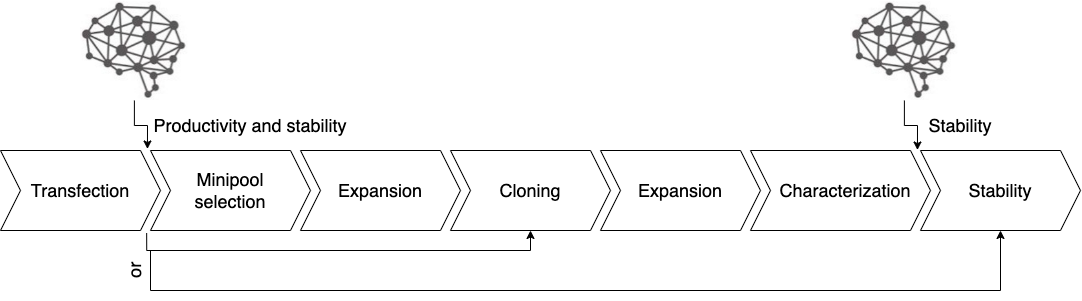
\includegraphics[width=0.8\linewidth]{bilder/CLD.png}
		\caption[CLD process steps]%
		{CLD process steps. Usual times needed for this process: from trnsfection to characterization --- 5 months, stability --- 3 months. Minipool selection step that is optimized here is taking up to 5 weeks.}\label{fig:cls-steps}
	\end{center}
\end{figure}

The first step of CLD is called transfection --- the introduction of the gene of interest (abbreviated as GOI or a DNA vector or, alternatively, an expression vector) into CHO cells. There are two main challenges with this step: firstly, transfection mostly results in a vector being inserted into a random site within the host cell genome and secondly, it generally has low efficiency of integration  (\cite{Tihanyi_2020}). It is important to transfect a GOI into the optimal site of the genome to secure high protein expression over time during protein production. Practically however, GOI is transfected into a random location of the genome. In cases where the gene was transfected into an inactive site of genome (essentially the majority of genome is transcriptionally inactive), the cell will likely be unable to express the gene (\cite{Castan_2018}, \cite{Hong_2018}).

%TODO [a better reference needed Shin 2020]
The second step of the process is the selection of cell minipools that have successful and stable gene integrations for further expansion and cloning. The reason for not all of them being suitable is that during the transfection step, only 80\% of the cells will receive a GOI vector (\cite{Castan_2018}). Only a small percentage of these cells actually integrate a vector into the genome and, as mentioned above, only a fraction of those are able to express the protein stably (\cite{Shin_2020}). After the best minipools are selected, they will be expanded.

The third step in CLD is to clone the cells. The selected stable pools of cells are phenotypically and genetically diverse. This means that they have different growth rates, metabolic profiles, and so forth. This is not ideal for industrial production - all the cells used for protein production should be derived from the same clone (\cite{ema_2020}). 

Once the cells are cloned, phenotypical and genetical heterogeneity is reduced, the next step is to characterize the cells for their expression of the GOI. One has to estimate the clones' productivity and stability. Such observations may take up to 90 days (usually stability measurements are made on the $30^{\text{th}}$, $60^{\text{th}}$ and $90^{\text{th}}$ days). If the clones remain stable after this time and are able to express enough of the protein, then they are suitable for further production. However, this last step is very time-consuming and requires maintenance for feeding and analysing the cells. Predicting productivity and stability of the cells in earlier stages would reduce this time significantly or even allow to avoid this process entirely.
        \subsubsection{Project specifications of cell line development for Merck KgaA}
        Description of my project, why is it useful, what are the processes here. How my neural network can be used for further stability predictions. My work as a part of the whole process of stability prediction
    \subsection{Deep learning and machine learning basics}
        \subsubsection{Neural networks}
            \begin{definition}[Image dataset]
	An image dataset in the scope of this thesis constists of input DIC images $X$ and target fluorescence images $Y$. Combined, couples from each form (X and Y) construct a dataset:
	\begin{equation}
		D = (X, Y) = \{(x^{(1)}, y^{(1)}), \dots, (x^{(N)}, y^{(N)})\}
	\end{equation}

	where both $x^{(i)}$ and $y^{(i)} \in \mathbb{R}^{W \times H}$ are single images, $N$ is the size of the dataset. Generally input data has a shape of $(N, C, H, W)$, in this work $C = 1$.
\end{definition}

\begin{definition}[Model]
	A model is a function with learnable parameters $\theta = (\theta_1, ..., \theta_K)$ where $\theta_i \in \mathbb{R}$ for $i \in {0, ..., K}$ which approximates the mapping of initial data $X$ to target data $Y$.
	\begin{equation}
		M(X,\theta) = Y^\prime \approx Y 
	\end{equation}
\end{definition}

\begin{definition}[Loss function]
	A loss function is a function $L(y, M(x, \theta))$ of model's parameters $\theta$, that for $(x^{(i)}, y^{(i)}) \in D$ outputs a scalar value measuring the difference between ground truth $y$ and prediction $M(x, \theta)$. A training objective is then defined as an average over the loss of each training sample:
	\begin{equation}
		J(\theta) = \mathbb{E}_{(x, y)\sim D} \left[L(y, M(x, \theta))\right]
	\end{equation}
	where $p_{data}$ denotes an empirical distribution of the training data.
\end{definition}

\begin{definition}[Weight initialization]
	Weight initialization is a process of setting the initial values of the parameters of a model to some random values.
\end{definition}

Weight initialization plays a crucial role in model training. Even on the simplest model wrongly initialized weights (for example all constant or too large or too small) can lead to very slow convergence or prevent the model from converging at all (\cite{Kumar_2017}).

In the following samples \textit{fan\_in} denotes the maximum number of input signal units to a given layer and \textit{fan\_out} is the maximum number of output signal units from it.

\begin{definition}[Xavier initialization]
	Xavier initialization, which is usually a default choice in many neural networks, works well for the most part for fully connected layers with tanh as activation function. There is also a study providing some insights into why Xavier initialization may not be the optimal choice for ReLU activations (\cite{Kumar_2017}). Xavier initialization draws samples from a uniform distribution:
	\begin{equation}
		Uniform \left(-\frac{1}{\sqrt{fan\_in}}, \frac{1}{\sqrt{fan\_in}}\right)
	\end{equation}
\end{definition}

\begin{definition}[He initialization]
	He initialization is another initialization method proposed by \cite{He_2015} as it was noticed that Xavier initialization is not an optimal choice for the networks that include ReLU activations. The authors suggest a new robust method that enables training of even extremely deep or wide network architectures with ReLU activations. He initialization draws samples from a truncated normal distribution:
	\begin{equation}
		{\cal N}(0, \frac{2}{\text{fan\_in}})
	\end{equation}
\end{definition}

Default weight initialization of Conv2D layers in Python suggests to use the following initialization method (\cite{He_2015}):
\begin{align}
	std &= \sqrt{\frac{2}{fan\_in}} \\
	bou&nd = \sqrt{3 * std} \\
	Un&iform\left(-bound, bound\right)
\end{align}

Although in the study of \cite{He_2015} it is called Kaiming normal initialization, it is a slightly different method.

\begin{definition}[Binary-cross entropy loss]
	Let $y \in \mathbb{R}^{W \times H}$ be a ground truth image and $y^\prime \in \mathbb{R}^{W \times H}$ be a prediction. Binary-cross entropy loss is defined as:
	\begin{equation}
		L(y, y^\prime) = - \frac{1}{N^2}\sum_{i=1}^{H} \sum_{j=1}^{W} y_{i,j} \cdot \log(y_{i, j}^\prime) +  (1 - y_{i, j}) \cdot \log(1 - y_{i, j}^\prime) 
	\end{equation}
\end{definition}

\begin{definition}[MSE (mean squared error) loss]
	Let $y \in \mathbb{R}^{W \times H}$ be the ground truth and $y^\prime \in \mathbb{R}^{W \times H}$ be the predicted images. The MSE loss is defined as:
	\begin{equation}
		L(y, y^\prime) = \sum_{i=1}^{H} \sum_{j=1}^{W} (y_{i, j} - y_{i, j}^\prime)^2
	\end{equation}
\end{definition}

\begin{definition}[PCC (Pearson correlation coefficient) loss]
	\label{def:pcc-loss}
	Let $y \in \mathbb{R}^{WH}$ be a flattened ground truth and $y^\prime \in \mathbb{R}^{WH}$ be a flattened predicted image. The PCC loss is defined as:
	\begin{align}
		PCC(y, y^\prime) &= \frac{\sum\limits_{i=1}^{{W\times H}}{(y_i - \bar{y})(y_i^\prime - \bar{y}^\prime)}}{\sqrt{\sum\limits_{i=1}^{W\times H}{(y_i - \bar{y})^2\sum\limits_{i=1}^{W\times H}(y_i^\prime - \bar{y}^\prime)^2}}}  \\
		L(y, y^\prime) &= \frac{1 - PCC(y, y^\prime)}{2}
	\end{align}
	where $\bar{y}$, $\bar{y}^\prime$ are means of the ground truth and predicted images respectively.
	
	There is an important distinction to be made here: firstly, Pearson correlation coefficient (PCC further) in a measure of similarity between two data sequences (matrices in this case), with values between $-1$ and $1$, with $1$ being a positive correlation, secondly, PCC loss is a measure of dissimilarity between two matrices, with values between $0$ and $1$, with $0$ meaning that matrices are the same.

	This loss is widely used in cell biology for comparison of co-localization between the proteins (\cite{Lachance_2020}). PCC is also popular in computer vision where it is utilized for the determination of image similarity in terms of spatial-intensity (\cite{Lachance_2020}).
\end{definition}

\begin{definition}[Optimization]
	Optimization is a process of updating the parameters $\theta$ of the model $M(X, \theta)$ to minimize the loss function $L(y, M(x, \theta))$.
\end{definition}

With a maximum likelihood esimation, we get:
\begin{equation}
	\theta_{MLE} = \argmax\limits_{\theta} \sum_{i=1}^{N} \log{p_{\text{model}}(x^{(i)}, y^{(i)}, \theta)}
\end{equation}

After maximizing the sum and taking a gradient one gets:
\begin{equation}
	\nabla_{\theta} J(\theta) = \mathbb{E}_{x, y \sim p_{data}} \left[\nabla_{\theta} \log{p_{\text{model}}(x, y, \theta)}\right]
\end{equation}

The exact gradient on a discretized data-generating distribution is then:
\begin{equation}
	g = \nabla_{\theta} J^*(\theta) = \sum_{x} \sum_{y}{p_{\text{data}}(x, y) \nabla_{\theta} L(y, M(x, \theta))}
\end{equation}

Here one can obtain an unbiased estimator of a true gradient on a mini-batch of i.i.d. samples $\{x^{(i)}, ..., x^{(m)}\}$	

\begin{equation}
	\hat{g} = \frac{1}{m} \nabla_\theta \sum_{i} L(y^{(i)}, M(x^{(i)}, \theta))
\end{equation}

\begin{definition}[Stochastic gradient descent]
	Stochastic gradient descent is an optimization algorithm where the parameters $\theta$ are iteratively updated every mini-batch of data by the following rule:
	\begin{equation}
		\theta_{k+1} = \theta_k - \alpha \frac{1}{m} \nabla_\theta \sum_{i} L(y^{(i)}, M(x^{(i)}, \theta))
	\end{equation}
	where $\alpha$ is a tuneable parameter called \textit {learning rate}.
\end{definition}

\begin{definition}[Adadelta optimizer]
	An Adadelta optimizer is a more sophisticated optimization technique, that follows algorithm \ref{alg:adadelta} for the parameter update.
	\begin{algorithm}[H]
		\caption{Adadelta optimization}\label{alg:adadelta}
		\item 1. $E[g]^2_0 = 0$ and $E[\Delta \theta^2]_0 = 0$
		In order to update the parameters one needs to:
		\item 2. Compute gradient: $g_t$
		\item 3. Accumulate gradient: $E[g]^2_t = \rho E[g]^2_{t - 1} + (1 - \rho)g_t^2$
		\item 4. Compute update: $\Delta \theta_t = \frac{\text{RMS}[\Delta \theta]_{t-1}}{\text{RMS}[g]_t} \hat{g_t}$
		\item 5. Accumulate updates: $E[\Delta \theta^2]_t = \rho E[\Delta \theta^2]_{t-1} + (1 - \rho) \Delta \theta^2_t$
		\item 6. Apply update: $\theta_{t+1} = \theta_t + \Delta \theta_t$ \\
		RMS here is the root mean square all initial hyperparametes are take from the original study(\cite{Zeiler_2012}).
	\end{algorithm}
\end{definition}

\begin{definition}[Adam optimizer]
	An Adam optimizer is another stohastic optimization technique, that has the following hyperparameters: $\alpha$ --- learning rate, $\beta_1, \beta_2 \in [0, 1)$ --- exponential decay rates. It follows algorithm \ref{alg:adam} for the parameter update.
	\begin{algorithm}[H]
		\caption{Adam optimization}\label{alg:adam}
		\item 1. Initialize: $m_0 = 0$ and $v_0 = 0$
		\item 2. Compute gradient: $g_t$
		\item 3. Update biased first moment estimate: $m_t = \beta_1 m_{t-1} + (1 - \beta_1) g_t$
		\item 4. Update biased second raw moment estimate: $v_t = \beta_2 v_{t-1} + (1 - \beta_2) g_t^2$
		\item 5. Compute bias corrected first moment estimate: $\hat{m_t} = \frac{m_t}{1 - \beta_1^t}$
		\item 6. Compute bias corrected second raw moment estimate: $\hat{v_t} = \frac{v_t}{1 - \beta_2^t}$
		\item 7. Apply update: $\theta_{t+1} = \theta_t - \alpha \frac{\hat{m_t}}{\sqrt{\hat{v_t} + \epsilon}}$
		Initial hyperparameters used in this work are $\alpha = 0.001$, $\beta_1 = 0.9$, $\beta_2 = 0.999$ and $\epsilon = 10^{-8}$.
	\end{algorithm}
\end{definition}

\begin{definition}[Overfitting]
	Overfitting is a phenomenon in which a hypothesis that fits training samples well will perform worse over the entire distribution on data rather than another hypothesis that fits the distribution of the training samples less well (\cite{mitchell_1997}). The way to avoid overfitting that happened to the models in Section \ref{section:er} are discussed in Section \ref{section:regularization}.
\end{definition}

\begin{definition}[Feedforward fully connected layer]
	A feedforward fully connected layer is a trainable function with parameters $W \in \mathbb{R}^{N \times M}$ (weights) and $b \in \mathbb{R}^{M}$ (biases) that, in this case, maps a vector $x \in \mathbb{R}^{N}$ to an output $a \in \mathbb{R}^{M}$ via the following transformation:
		\begin{equation}
			a = W^{T}x + b
		\end{equation}
\end{definition}

This is one of the simplest layers in a feedforward neural networks and input and output in it as mentioned above are vectors. However, in this study inputs and outputs are images, that are represented in memory as square matrices $x^{(i)}, y^{(i)} \in \mathbb{R}^{N \times N}$. One could simply flatten the image into a vector and use it as an input to a fully connected feedforward neural network. Nevertheless this would be a suboptimal approach. 

Since essentially one of the main tasks of this research is to create a deep learning model that is able to predict a fluorescence image from a DIC image, the problem statement could be narrowed down to the following: predict an intensity high-resolution image from another intensity high-resolution image based on the features of the object morphology in it. Such problem is very common in the field of image analysis and one of the popular deep learning tools for solving such problems is convolutional neural network (CNN) or more specifically a UNet.

CNNs are able to capture nonlinear relationships over large areas of images, they greatly improve performance for image recognition tasks in comparison to classical machine learning methods (\cite{Ounkomol_2018}). The word "convolutional" suggests that the convolution operation should be used in at least one of the layers there.  

\begin{definition}[Convolutional layer]
	A convolutional layer is a trainable function with parametrized kernel $K \in \mathbb{R}^{F \times G \times C}$ and bias $b \in \mathbb{R}$ that is usually denoted via the operator $(\cdot * \cdot)$. By transforming an input $x \in \mathbb{R}^{W \times H \times C}$ it produces an output $S$
	\begin{equation}
		S = K * x + b
	\end{equation}

	that is called a \textit{feature map} where an element on position $(i, j)$ is defined as follows:
		\begin{equation}
			S_{i, j} = \sum_{w} \sum_{h} x_{m, n}  K_{i - m, j - n}
		\end{equation}
\end{definition}

Convolutional layer like a fully connected layer can be viewed a linear transformation as well. However, there are three main advantages that leverage convolutional layers for image processing in comparison to fully connected layers: sparse interactions, parameter sharing and equivariant representations. An image is a very redundant way of representing the semantic meaning hidden within it. Having a value of one pixel, the probability that the neighboring one will be of the same color is very high. Sparsity of interactions can be described by an example: usually a high-resolution image might have millions of pixels, however it is possible to detect smaller and very important features like contrast changes, edges, and shapes using a kernel consisting of only a few hundred pixels. By applying kernels (or filters) on the image locally, one will infer many of these features across the whole image. Such an approach reduces the memory needed for parameter storing and improves its statistical efficiency (\cite{Goodfellow_2016}). Parameter sharing refers to the fact that instead of learning a separate set of parameters for every location within the image, only one set of parameters will be learned and applied across all image locations. Lastly, equivariance here means that convolution operation is equivarient to the shifts in the image.

\begin{definition}[Stride]
	During the computation of convolution, the kernel starts sliding at the upper left corner of the input tensor, covering all locations while heading to the right and down. The step with which the window slides is called \textit{stride}. 
\end{definition}

\begin{definition}[Padding]
	When convolution is applied several points on the perimeter of the input tensor will be lost and the ouput tensor will have smaller spatial dimension than the input one. One can fix this by adding a few more pixels outside the perimeter, to preserve the dimension of the output to be same as input. The amount of pixels added is called \textit{padding}. 
\end{definition}

Visual examples of what stride and padding represent are shown in Figure \ref{fig:stride}.
\begin{figure}[htb]
	\begin{center}
		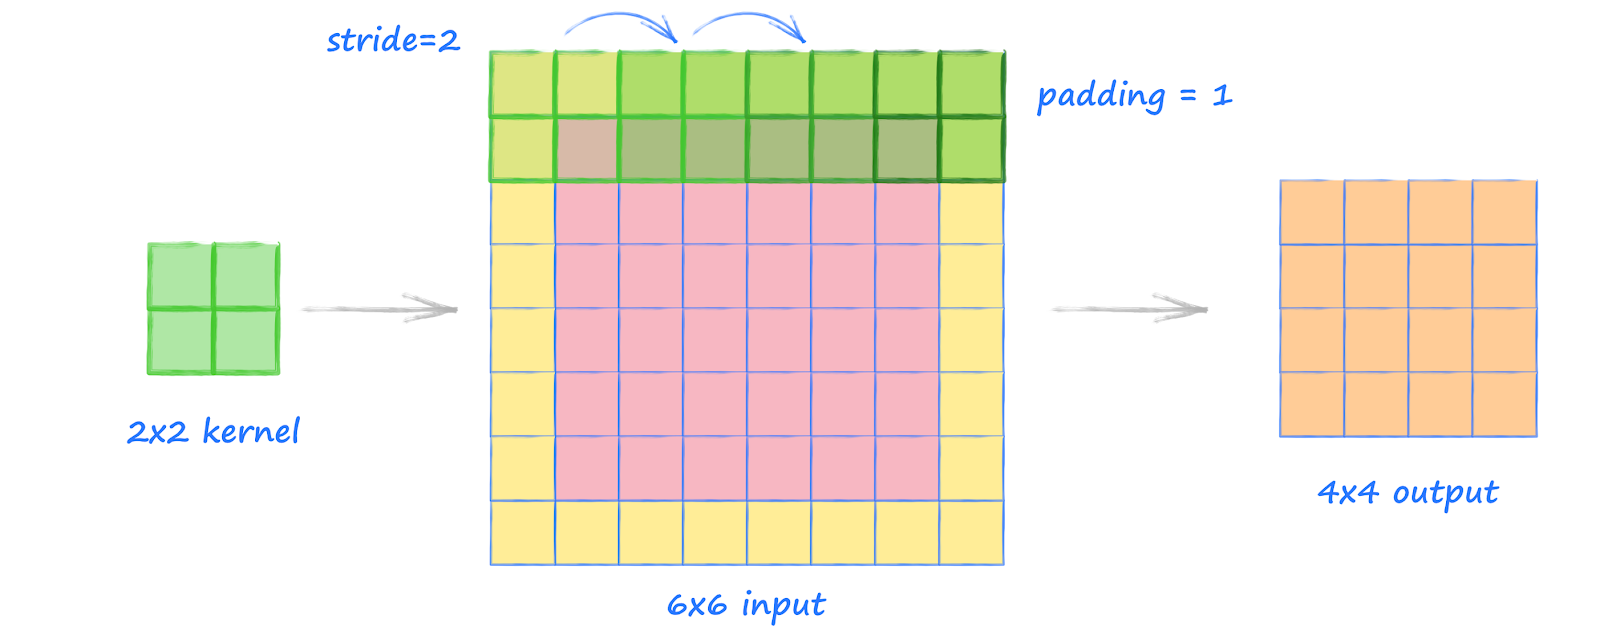
\includegraphics[width=0.6\linewidth]{bilder/stride_padding.png}
		\caption[Stride and padding example]%
		{Stride and padding example. Taken from \cite{stride}.}
		\label{fig:stride}
	\end{center}
\end{figure}

\begin{definition}[Max-pooling layer]
	Maximum pooling operation reports the maximum output within a rectangular neighborhood (\cite{Goodfellow_2016}).
\end{definition}

\begin{definition}[Activation function]
	An activation function is an element-wise non-linear function $f(\cdot)$. Some examples are:
	\begin{align}             
		f(x) = \frac{1}{1 + e^{-x}} &&\text{Sigmoid} \\      
		f(x) = max(0, x) &&\text{Rectified linear unit (ReLU)}\\
		f(x) = \begin{cases}
				x, \hspace*{1cm} \textrm{if } x > 0 \\
				\alpha * (e^{x} - 1), \textrm{if }  x \leq 0
		  	\end{cases}\ &&\text{ELU}
		\end{align}
\end{definition}

It is important to use activation functions after each convolutional or linear layer like RELU, ELU, Tahn, Sigmoid or any other non-linearities. Because any combination of linear functions can be represented with another linear function, having consecutive linear layers without non-linear function in the network is equivalent to having just one linear layer. Non-linearities  In CNNs they are also often combined with max-pooling layers and dropouts to escape overfitting. 

\begin{definition}[Batch normalization layer]
	Let's denote $B = \{x^{(i)}, ..., x^{(m)}\}$ to be a mini-batch of data. Then batch normalizing transform applied to this input data would be:
	\begin{equation}
		\begin{split}
		& a^{(i)} = \gamma \frac{x^{(i)} - \mu_B}{\sigma^2_B + \epsilon} + \beta \\
		& \sigma^2_B = \frac{1}{m} \sum_i^m (x^{(i)} - \mu_B)^2 \\
		& \mu_B = \frac{1}{m} \sum_i^m x^{(i)} \\
		\end{split}
	\end{equation}
	where $\gamma$ and $\beta$ are learnable parameters, $\mu_B$ and $\sigma^2_B$ are the mean and standard deviation of the batch (\cite{Ioffe_2015}).
\end{definition}

\begin{definition}[Dropout layer]
	Dropout is a technique that randomly sets some weights (units) to zero (\cite{Srivastava_2014}). It leads to the training of several smaller networks that share the parameters. If a mask vector $\mu$ specifies which units are included in training, then dropout's objective to be minimized becomes: $\mathbb{E}_\mu \left[J(\theta, \mu)\right]$. Visually dropout is presented in the Figure \ref{fig:dropout}.
\end{definition}

%TODO add figure reference!
\begin{figure}[H]
	\begin{center}
		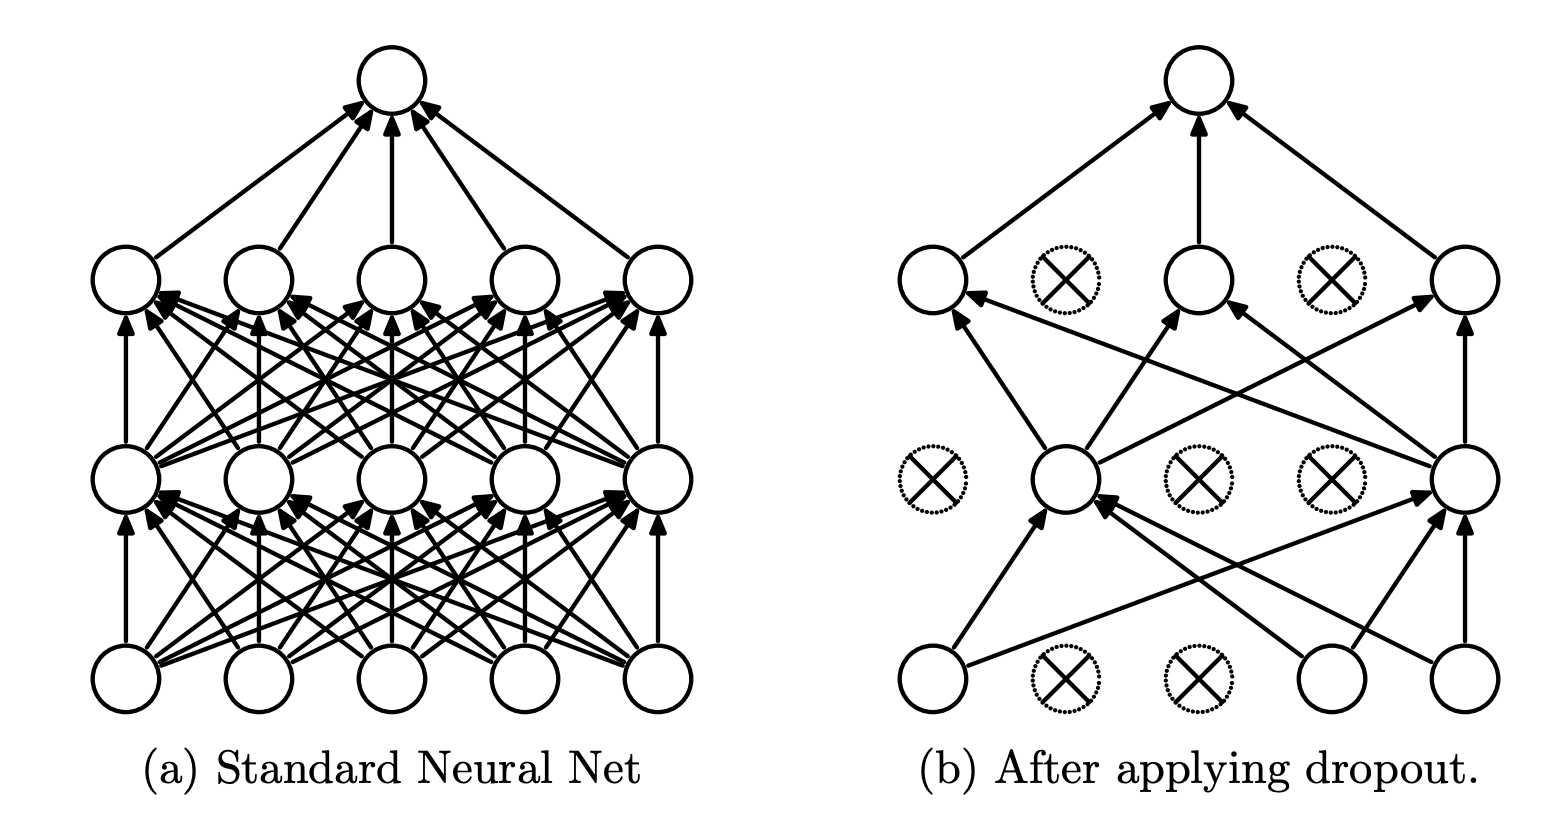
\includegraphics[width=0.5\linewidth]{bilder/dropout.png}
		\caption[Dropout]%
		{Dropout. Taken from \cite{Srivastava_2014}}
		\label{fig:dropout}
	\end{center}
\end{figure}

The models in this project mostly use ELU activations as ELU provides a better signal flow between the layers by not cutting off the negative values completely.

\begin{definition}[UNet]
	UNet is fully convolutional neural network with U-shaped encoder-decoder network architecture (\cite{Ronneberger_2015}). Example of the UNet architecture can be found in Figure \ref{fig:unet}.
\end{definition}

The encoder is a common CNN, consisting of the repeated
block of two $3 \times 3$ convolutions, followed by
an activation function, and a $2 \times 2$ max-pooling operation with stride 2. At each encoder step  the number of feature channels doubles. The decoder is also a CNN, consisting of repeated blocks of transposed convolution, that halves the number of feature channels, followed by a concatenation with a corresponding output from an encoder, and two $3 \times 3$ convolutions, followed by a ReLU. The last decoder layer is a $1 \times 1$ convolution to map the tensor to the number of output image channels needed. Skip-connections is a very important part of UNet as they allow to the flow of high-resolution features from the encoder to the decoder that in turn allows to restore a corresponding high-resolution image.

\begin{definition}[Autoencoder]
	Autoencoder is an unsupervised learning technique in neural networks for the representation learning purposes. Autoencoder consists of an encoder that compresses data into a lower dimensional representation and a decoder that restores the original input from the encoded representation.
\end{definition}

\paragraph{Regularization techniques}
\label{section:regularization-theory}
% TODO add overfitting image?
Regularization is mostly used to prevent a deep learning model to overfitting on the training data and to be able to generalize well. Overfitting has occured in the models used in this research and therefore it is improtant to understand the techniques that can be used to prevent it. There are are several approaches to regularize the model and they will be explained below.

\begin{itemize}
	\item Early-stopping

	Overfitting can be detected via visualizing train and validation losses. Training behaviour at first will be the usual one, meaning that both train and validation losses are gradually decreasing, however at some point the train loss continues to decrease, whereas the validation loss suddenly starts to increase. Since the model has not seen any of the data from the validation set, it means that it loses its ability to generalize on unseen data, while improving its perfomance on the seen data (train set). This does not happen during earlier epochs. Assuming that the model learns a complex decision surface while training, the weights of the model will be quite small and random with the correct weight initialization and therefore the best decision surface during the early epochs would be a smooth one. But during the later ones the difference in values of the weights grows and they become dissimilar which also means that the decision surface becomes more complex and the model is now able to fit not only the training data itself, but also its noise (\cite{mitchell_1997} p.111). And that is why stopping before the model becomes too complex, meaning to stop before the overfitting point, mitigates this problem.

	\item \emph{L1}- \emph{L2}-regularization

	The complexity of the deep model grows with the number of features it uses, sometimes the model may pay attention to the features that are not important to the outcome, or even considers noise to be a feature. To prevent this one should decrease the weights associated with useless features, however one cannot know ahead of time which of them should be ignored, therefore one may limit them all (\cite{Ying_2019}). In order to do that, a penalty term is added to the loss function:

	\begin{equation}
	\tilde{L}(Y, M(X, \theta)) = L(Y, M(X, \theta)) + \lambda R(\theta)
	\end{equation}

	for some $\lambda > 0$. This is called a \emph{soft-constraint} optimization. When $R(\theta)$ is of the form $R(\theta) = ||\theta||^2_2 = \sqrt{\sum\limits_i \theta_i^2}$ this is called \emph{L2}-regularization. When it is of form $R(\theta) = ||\theta||_1 = \sum\limits_i |\theta_i|$ this is called \emph{L1}-regularization. \emph{L2}-regularization used in combination with backpropagation is equivalent to weight decay. Weight decay is defined by \cite{Hanson_1988} as follows:
	\begin{equation}
		\theta_{t+1} = (1 - \lambda)\theta_t - \alpha \frac{\partial L}{\partial \theta_t}
	\end{equation}

	where $\alpha$ is a learning rate. Weight decay successfully has more effect on the weights along which the gradient change is smaller \cite{Goodfellow_2016}. \emph{L1}-regularization induces sparsity of the weights by assigning some of them to zero, this could also be considered as a feature selection approach.

	\item Regularization layers

	Batch normalization and dropout layers are also considered to be a form of regularization.

	\item Network reduction

	Since learning a too complex and noise-fitting decision surface might be a frequent cause of an overfit, another way to mitigate this would to be reduce the space of the possible decision surfaces and therefore make the surface simpler so that it cannot fit into the noise from the data. By changing the number of adaptive parameters in the network, the complexity can be varied (\cite{Bishop_2006} p.332).

	\item Expansion of the training data

	For a successful training a model needs to have a sufficient amount of quality samples. An expanded dataset can improve the quality of the predictions \cite{Ying_2019}, however only when the model has already performed well on the initial dataset. If the model was performing badly initially, adding more data will not solve the problem.
\end{itemize}

        \subsubsection{Dimensionality reduction methods}
            This reseach additionally provides the study of the embeddings of a trained UNet and an Autoencoder in Chapter [TODO cite chapter]. In order to understand the visualizations better all dimensionality reduction methods that were used here are listed and explained in this subsection.

\begin{definition}[Embedding]
    An embedding in this context is an output tensor from the encoder part of the UNet or from an encoder part of an Autoencoder.
\end{definition}

The encoder output of the UNet is a tensor of size $16 \times 16 \times 256$ and after its flattening it turns into a vector of size $655536$. The smallest autoencoder embedding was of size 200 [TODO check] which is also high-dimensional. One of the tasks of this research if to determine wethere there are any interesting patterns or grouping based of various criteria hidden within the bottleneck embeddings, and wether they could be useful for further research. Yet in order for humans to comprehend the embeddings we need to maps them either to 2D or 3D vectors and that is where dimensionaluty reduction algorithms are essential.

\paragraph{UMAP}
Dimension reduction algorithms mostly form two main categories: ones are stronger preserving the pairwise
distance globally - meaning try to preserve the structure amongst all the data samples; others prefer to save local distances. For example PCA [cite Hotelling] are assigned to the first caterogy, while t-SNE [cite Ulyanov] and Isomap are assinged to a latter one.

Uniform Manifold Approximation and Projection (UMAP) was build in a way to preserve both and it is a competitor of t-SNE approach, however is much faster and provides a transformation that can be used on the new data. UMAP is a graph-based algorithm and uses a k-nearest graph as a foundation. As any graph-based algorithm, its structure also includes two main steps: 

%[TODO need a synonym instead of ambient == surround]
\begin{itemize}
    \item Graph construction procedure. During this stage a weighted k-neighbour graph will be constructed from the data. Specific transformation are applied on its edges to surround local distance. And the strong asymmetry common to k-neighbour graphs will be reduced.
    \item Graph layout building. In this stage one needs first to define an objective function that can preserve desired graph characteristics and then find a low dimensional representation of the graph that will minimize the objective.
\end{itemize}

%https://pair-code.github.io/understanding-umap/
In short, UMAP optimizes a low-dimensional graph from the high-dimensional one to be structurally very similar to each other. The algorithm has to important hyperparameters, which should be chosen carefully: \textit{n\_neightbors} and \textit{min\_dist}. The first one balances the local versus the global structure of the graphs, the higher the values the more finer details will be lost. The latter one controls how densly points will be located to one another. Higher values of this parameter results in a loosier structure that preserves a broader topoly of the data. 

\paragraph{PacMAP}
Pairwise Controlled Manifold Approximation (PacMAP) is another dimensionality reduction method that is able to preserve both local and global data structure in a lower dimension space. Unlike other methods that regulate the stronger preservance of global structure by using more neightbors, PaCMAP uses mid-near pairs, to first capture global structure and then refine local structure, which both preserve global and local structure. It introduces a the following parameters: neighbor pairs (pair\_neighbors), mid-near pair (pair\_MN), and further pairs (pair\_FP). [cite Yingfan] The neighbor pairs parameter is used during the building of the k-Nearest Neighbor graph. It is recommended to use the value around 10 for datasets with size smaller than 10000 [cite their repo]. The mid-near pair ratio parameter is the ratio of the number of mid-near pairs to the number of neighbors, whereas further pairs ratio is the the ratio of the number of further pairs to the number of neighbors. Configuring these parameters allow the user to achieve the desired ration between preserving local and global structure. Such method also works faster than UMAP, which allows to try out more hyperparameter options.

\paragraph{PCA}
Principal component analysis (PCA) is an algorithm for linear dimensionality reduction [cite Pearson 1901].  PCA maximizes the variance in data's low-dimensional representation in order to keep as much information as possible. Essentially PCA gives projections $\tilde{x^{(i)}}$ for input samples $x^{(i)}$ that would be very similar to them, however have a much smaller dimensionality. Eigenvectors of the data covariance matrix are the directions of the most variance within the data, and the eignevalues correspoding to them are the amount of variance hidden in each dimension. That is why by projecting the data using the eigenvectors with the largest eingenvalues one will preserve the most varience of the data possible [cite MML-book].

The steps of PCA algorithm are the following:
\begin{itemize}
    \item Subtract mean $\mu_d$. To center the input data is not a nessesary step, but it is recommended to do so to avoid the numerical problems.
    \item Standartize the data. Calculate the standard deviation $\sigma_d$ and standartize the data to have unit variance for every dimension. 
    \item Do an eigendecomposition of the data covariance matrix. For that one first must compute the coveriance matrix itself, since the covariance matrix is symmetric from the spectral theorem one can always find an orthonomal basis of eigenvectors. 
    \item Project the data. For that first standartize the point $x^* \in \mathbb{R}$ using $\mu_d$ and $\sigma_d$:
        \begin{equation}
            x^*_d  \leftarrow \frac{x^*_d - \mu_d}{\sigma_d}
        \end{equation}
        where $d = 1, ..., D$ and $x^*_d$ is a $d$-th component of vector $x^* \in \mathbb{R}^D$
    Get the projection as 
    \begin{equation}
        \tilde{x^*} = BB^T x^*
    \end{equation}
    with coordinates $z^* = B^Tx^*$. Here $B$ is a matrix of eigenvectors associated with the biggest eigenvalues of a covariance matrix.
\end{itemize}
[cite MML-book]
        \subsubsection{Clustering}
            \paragraph{DBSCAN}
\paragraph{HDBSCAN}
\paragraph{K-means}
    \subsection{Imaging}
        \subsubsection{Digital imaging}
            Digitally an image is represented as an array of size $(H, W, C)$ where $H$ is the height, $W$ is the width and $C$ is the number of channels of the image. In this work, $C = 1$ and $W = H$. A digital image $A$ can be    represented with the matrix:

\begin{equation}
    A = \left[
            \begin{array}{ccc}
                a_{0,0} & \cdots & a_{0,W-1} \\
                \vdots & \ddots & \vdots \\
                a_{H, 0} & \cdots & a_{H-1, W-1}
            \end{array}
        \right]
\end{equation}
where $a_{i, j} \in \mathbb{R}$. Both DIC and fluorescence images were provided in tag image file format (TIFF). For the processing convenience purpose all images were normalized to be in the range of $[0, 1]$:

\begin{equation}
    a^{\text{norm}}_{i,j} = \frac{a_{i, j} - \min(A)}{\max(A) - \min(A)}
\end{equation}
for $ \forall i \in \{0, ..., W - 1\}$ and $ \forall j \in \{0, ..., H - 1\}$
            How image is stored in memory, which conventions there are (RGB, BGR (conventions are used in corruptions augmentations)).
        \subsubsection{Microscopy imaging}
            \paragraph{Image acquisition peculiarities}
    The cells used in this research are growing in 96-well plates. A plate or a microplate in biology is a flat plate with multiple tubes ("wells"). The microscope used in the experiments takes photos of the well plate in random locations. The reason for that hides in the focusing settings of a  microscope.  To get a reasonably good, and not blurry, photo, a microscope has to focus on a specific location of the plate. The choice of this location however happens automatically, therefore the location of the focus is random (see Figure \ref{fig:random-dic}).

    It might be problematic in the following sense: photos taken in such a manner do not guarantee that the focus will land in distinct spots all the time. Meaning that some cells present in one of the photos might appear in the other ones as well. Since the photos are high-resolution they will first be split into crops of size $256 \times 256$ each during the preprocessing. It might happen that the same cells appear in several crops. That is why after the split of the image data between train, test and validation sets it might also happen that the same set of cells will once land in the train set and another time in the validation set, which will lead to a not completely fair and representative validaiton metrics during training.

    In order to overcome this problem much more expensive equipment is needed. Since it does not cause fundamental problems in this case, except for the fact that the validation metrics might be lower than what they should have been, there was no need to purchase more expensive tools.

    \begin{figure}[htb]
        \begin{center}
            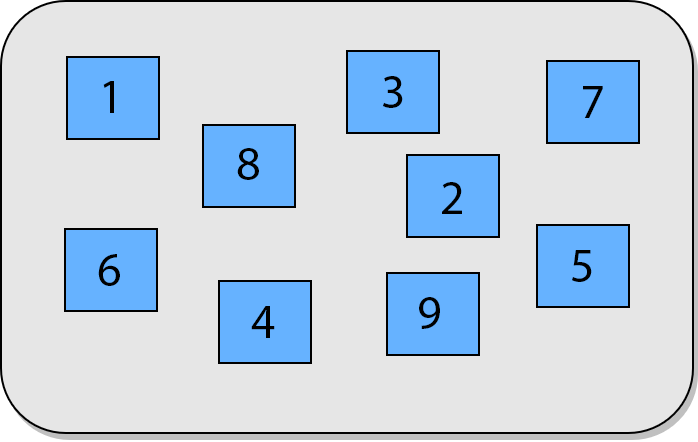
\includegraphics[width=0.6\linewidth]{bilder/dic-random.png}
            \caption{Way in which photos of the well-plate were taken}\label{fig:random-dic}
        \end{center}
    \end{figure}
\paragraph{Crops combination technique}\label{par:crops-combination}
    Due to the restricted amount of memory on the GPU deep learning models cannot have a high-resolution image as their input in the scope of this research. Yet this is also not obligatory: as the image contains dozens of cells within it, its processing can be limited to a crop of a smaller size. After the model has predicted fluorescence signal for each of the crops, output fluorescence images can be combined together to form a high-resolution image again. In this thesis the architecture of the model assumes an input size of $(256, 256)$ or more specifically $(None, 1, 256, 256)$, where the first dimension is responsible for the batch size and the second one states that the input is a 1-channel image. 

There are several ways of how one can split the image, the easiest approach would be to use a sliding window of size $w$. This algorithm is depicted in Figure \ref{fig:sliding-window}. A small window starts sliding the image from the upper left to the lower right corner with step size $s$ feeding the selected crops into a deep learning model. From the output of the model only a center part of such a crop is accepted to form a full fluorescence image. Border size $b$ in this case is the size of the edges of the crop that are not accepted from the predictions of the deep learning model.

Accepted areas from each of the crops have to follow each other without any space in between. In oder to achieve that if the border size has been defined in advance, one has to set the step size to in the following way:
\begin{equation}
  s = w - 2 * b
\end{equation}
When step size $s$ is equal to window size $w$, there is no overlap between the windows.

\begin{figure}[H]
	\begin{center}
		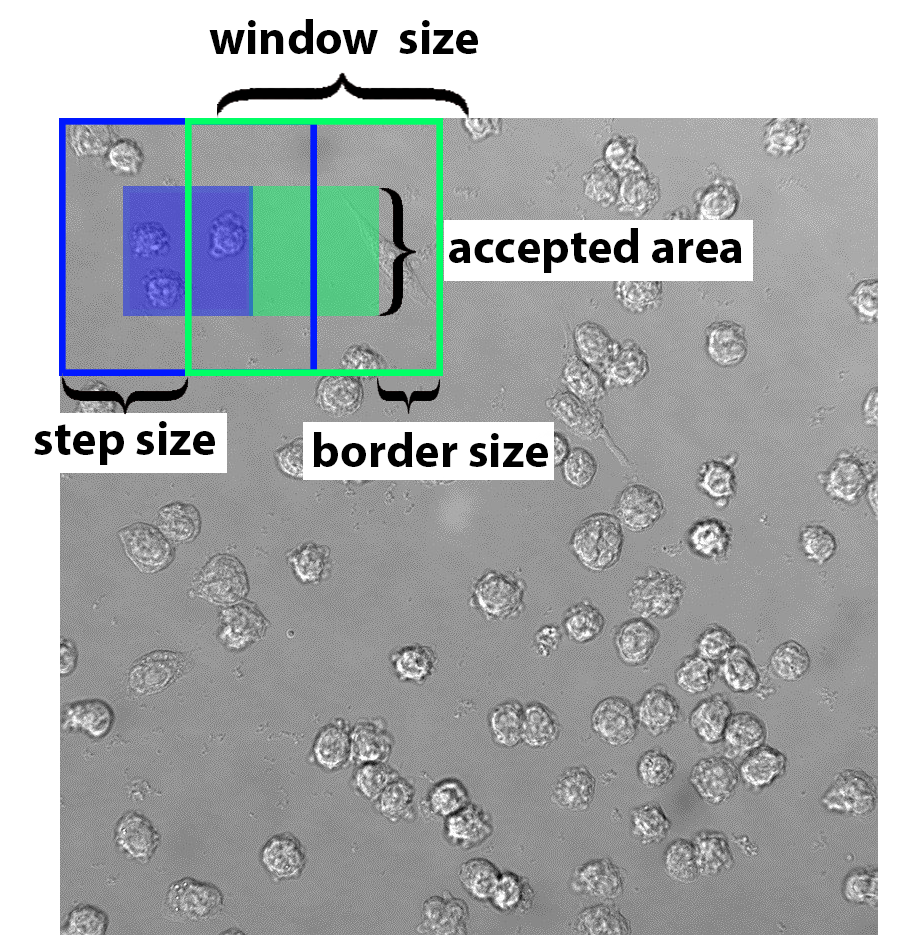
\includegraphics[width=0.3\linewidth]{bilder/sliding-window.png}
		\caption{Sliding window approach for fluorescence prediction}\label{fig:sliding-window}
	\end{center}
\end{figure}
The reason why the full prediction is not accepted to form the output lies in the following: trained models are less accurate on the borders of the crops rather than in the center. Most of the times there are cells on the borders of the crops that were sliced and therefore it might be impossible to make a good prediction for them just due to the lack of input information. Therefore, the step size has to be smaller than the window size, so that the windows are overlapping and for each prediction we use only the image center and are allowed to ignore predictions on the border (see the comparison between different border sizes in Figure \ref{fig:crops-combination}). This is discussed in more detail in Section [TODO reference the section]. Such an approach helps to reduce the effect of grid visibility on the image composed of many small crops. This can be seen in the left part of Figure 5 as opposed to the non-visible borders in the same Figure on the right. This would of course take more time to created the predictions, however, the speed is less crucial in comparison to the accuracy of the predictions.

\begin{figure}[htb]
	\begin{center}
		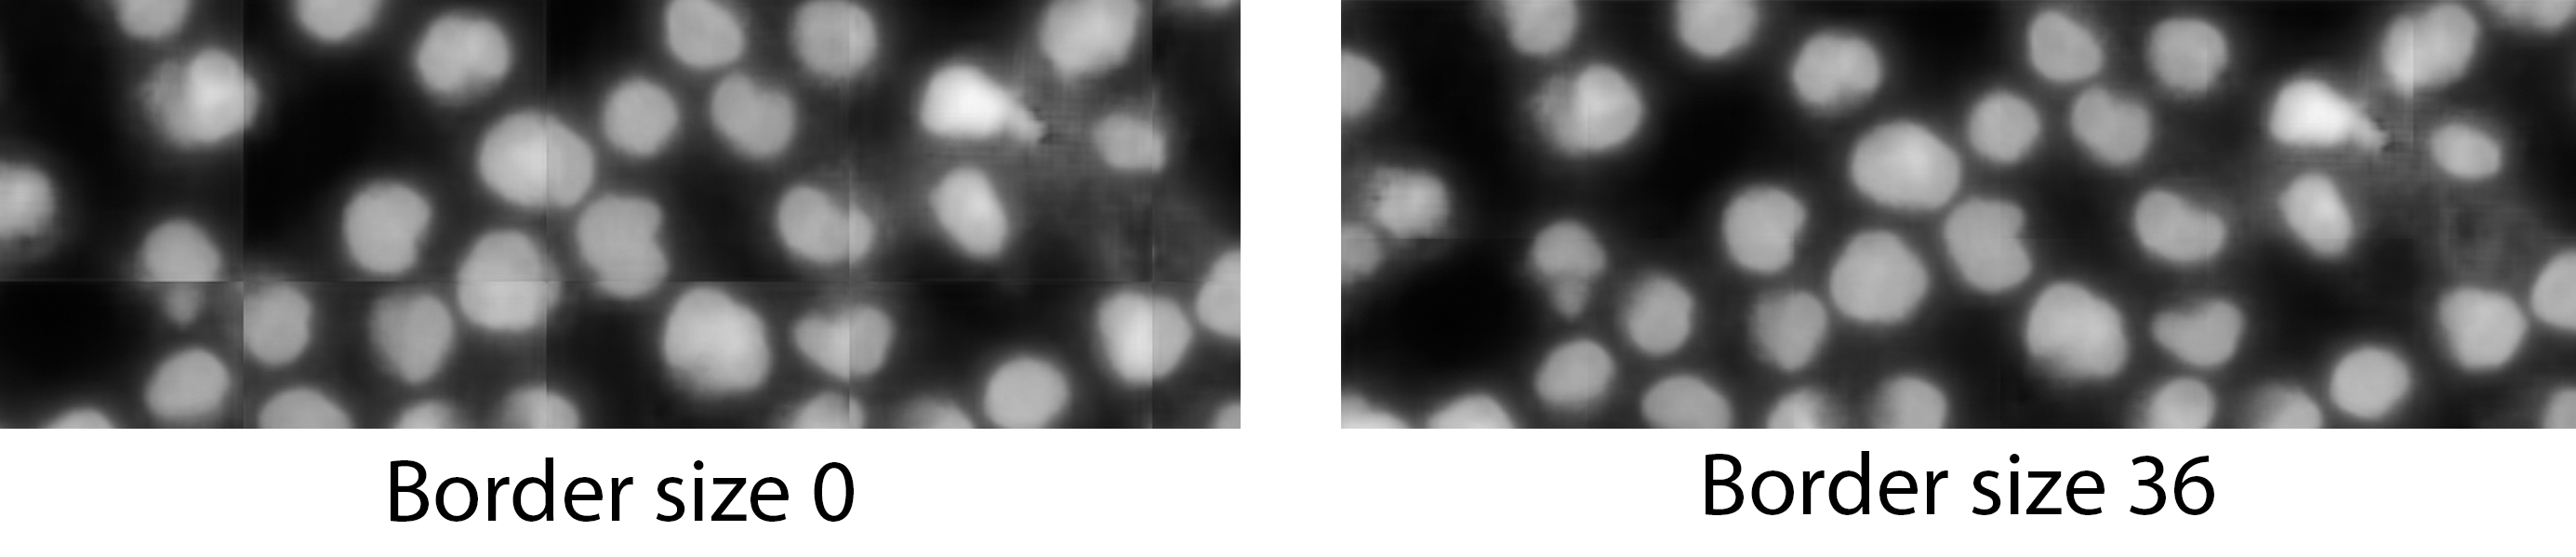
\includegraphics[width=\linewidth]{bilder/crops_combination/crops-combination.png}
		\caption{Difference of overlap between predictions on the resulting image}\label{fig:crops-combination}
	\end{center}
\end{figure}
